% Implementation design :


% TODO Denne må skrives heilt om. Sett av to dager til dette. (1 natt+en dag?)


%XXX INNLEDNING til kap. ER FLYTTA TIL rapport.tex (ELLER er planlagt flyttet).
	% Skrive at alt dette er egenprodusert. Alle mekansimer, ligninger osv er egenprod. Dette var unødvendig, da SANN allerede er laget. Det er difor mulig at eg har innført nokre nye element for dette.
		% Siden alt er egenprodusert ("oppfinne hjulet på nytt") har eg ikkje leita mykje om implementasjonsspesifikke detaljer, og det er lite referanser i dette kapittelet.

% 			Først: Innledning FOR KAPITTELET.
% - Skriv at for å gjøre restultata mest sammenlignbar, så tenkte eg initiellt at signalet propagerer ved "fyring" for begge modellane (KANN og SANN). Dette er gjort om.
% - Nevn forskjellane: SANN ser på tilstanden, mens KANN ser på tilstand+input for å beregne fremtidig fyringstid. Dette fører til behovet for pEstimatedTaskTime. Beskriv behovet. Mulig bruk i SANN også..
%  		(dette vil bli sett på i section {secSANN} og {secKANN}).
% - Læring (syn. p.) er ikkje implementert pga. tidsbegrensninger(og  siden dette ikkje er en del av oppgaven).							= "For further research".
% 		- Blir dermed sammenligning av to modeller for å designe `recurrent ANN': "Moore vs. Mealy state maschine of the biological neuron".
% - Siden målet er å beskrive forskjellane i implementasjonen, er det viktig å isolere forskjellane mest mulig.
%  		-> Dette vil bli diskutert i section ? (secSammenligningDesign?)
% - For sammenligning av enkeltnodene er det best å ta bort så mange variabler som mulig. Difor er eit kaotisk neuralnett som input uakseptabelt.
%  		Løsninga blei å igjen hente inspirasjon fra biologien, og lage eit spesialisert "sensor neuron". Dette skal bare nevnes her, og TODO skrives eit avnitt av seinare i kap.
% 		Dette blir designet i section [secSensorNeuronDesign?].

% 				- Til innledning:  Sjå "kladd fra tidligare: effektivitet". Om at det er vanskelig å forutse kva som er effektivt. Eit par gode poeng der. Bør teste effektivitet, men dette får bli "for futher research".


%XXX section design
% 				- About efficiency (om å optimalisere effektivitet. Kø for beregning. (Variant av) avsnitt er skrevet)
% 			skriv om sensor funksjoner!
% 				- loggføring - sjå "log for comparison".
% 				- synaptisk plastisitet. Har ikkje tid. Skriv at vi i denne oppgava fokuserer på implementasjonsforskjellen mellom KANN og SANN. Dersom effektivitet skulle sammenlignes er det best å fjærne syn.p. fra ligninga (mindre kaos)
% 				- Skriv om kvalitative forskjeller for SANN og KANN. Forskjellen mellom SANN simulering av neuron og KANN matematisk simulering med estimering til fremtida.







% 	Section: Design.
% 		- Time
% 		- The object design
% 		- Oppbygging av to typer ANN ved arv.
% 		- Om effektivitet
% 		- Om oppsamling av K
% 		- Syn. P.
% 		- Log for comparison
%
%
%
%i subsection "sammenligning" (også noko som må designes..):
% 		%- Tenkte initiellt å sammenligne effektivitet. Dette blir ikkje tid til.
% 		% 	Målet blir heller å utvikle og sammenligne KANN mot SANN, ikkje resultatet av kjøringa av de to (ikkje effektivitet, men andre aspekt..) Dette bør kanskje skrives om.
% 		%- Siden målet er å beskrive forskjellane i implementasjonen, er det viktig å isolere forskjellane mest mulig.
% 		%	- Lager dermed eit generellt rammeverk som gjelder for begge implementasjonane, og modellane som underelement av elementa:
% 		%		Underklasser av kvart element i nodene (SANN og KANN) som arver fra felles i_[element] abstrakt klasse. Dette gjør det lettare å isolere forskjellane (mest mulig av det som er likt ligger i i_[element]).


% TODO Skriv om sensor funksjoner!




\section{Design} % eller "Design; General Consepts for both Imlementations" eller noke anna..
	\label{secDesignForANN}
	% Skriv en liten innledning til denne section. Det er tross alt litt tekst i den..

	%In this section the common framework of the design and implementation of the two models will be presented.
	%TODO Gå gjennom opplistinga i neste linje, når section er ferdigskrevet.
	This section will start with describing the common framework of the implementations; 
		General concepts such as simulated asynchronicity (sec.\ref{ssecTime}), generality of the implementation and the design of the indivitual node will be presented in this section. %TODO sett på internreferanser til rett subsection.
	After the common framework of the simulation is presented, there will be a short discussion about how the two simulators are distinguished. %TODO skriv om! slutten er dårlig
	%Towards the end of the section, different aspects like efficiancy and generality of the implementations are presented
	A method for time scheduling is introduced in sec. \ref{secPlannedEvents}.
	% XXX
	Finally, concepts that are important for the comparison between the transient time course of the two models will be introduced is sec. \ref{ssecLogForComparison} and sec. \ref{ssecTheSensorNode}.
	
	
	%The ide is that a simulation based on higher level mathematics gives a more effective execution of the ANN than a direct simulation of a biological system.


	%   (Husk:  etter bra innledning har eg og leseren samme utgangspunkt i følgande subsections).


	\subsection{Time}
	\label{ssecTime}
	The biological neurons does its tasks completely asynchronously.
	%The concept of ``asynchronous'' comes from electronics, where 
	By this it is ment that the different mechnanisms of one neuron can happen independently from an other, and the effectivity of one is not affected by the workload of other neurons.
	This causes the calculation at each node to happen independently of other neurons.
	%By this it is ment that the excitation, inhibition and firing of one neuron is separated from other neurons; %Ikkje "separated", men adskilt
	%	Multiple neurons can do theire tasks simultaneously with no loss in efficiancy.
	%One neuron can therefore be excited to suprathreshold values without affecting the efficiancy of other neurons, and multiple tasks can be done simultaneously.
	%One neuron can therefore be excited to suprathreshold values and fire without affecting the efficiancy of other neurons' calculation. 


	In the computer, tasks are performed serially in one or multiple processors.
	To simulate the same degree of asynchronous behavior, time also has to be simulated. %TODO Skriv om litt.
	The consequence is what will be referred to as simulated asynchronicity.
	%This will in the remainder of this text be referred to as simulated asynchronicity.
	%To get the same degree of asynchronicity in simulated neurons, time will also have to be simulated.

	In digital electronics, asynchronous design refers to clockless circuits. 
	With respect to time, every part of the circuit executes its task independently of other parts.
	%Every part of the circuit executes its part independently of the other, in respect to time.
	This interpretation of the concept is not possible to accomplish in the serial processor; Tasks can per definition not happen serially, independent of the timing of the other processes.
	The solution to this is to let the time in the simulation be simulated.
	As time (``chronos'') becomes a variable that is under our control, it is also possible to control chonology in the simulation. %XXX ".. under our contro." => ".. under the implementation's control."
	This means that the simulator is able to arrange the order of events in theire order of occurence in the simulated time. %TODO ÆRS! Krokete som helvete. KRØKETE SKREVET: Skriv om!
	%It is therefore possible to control the order of the events in the order of theire order of occurence in time, in the simulation.
	
	In a simulation of tree nodes, node B can therefore be scheduled to fire after node A but simultaneous to node C.
	%The consequence of this is that in a simulation of a network of tree nodes, node B could be ordered to happen after node A but simultaneously to node C, in respect to the simulated time. %Litt dårlig. KRØKETE
	As each node has a time variant value due to ``leakage'', time is an important element of the mechanisms of each node.
	%As each node has a time variant value, with a value that leaks in respect to time, time is a very important element of the mechanisms of each node.
	The concept of simulated time therefore becomes very important for the simulator. 

	The simple solution to the concept of simulation of time, is to iterate through all nodes at each time step, and update the nodes' value.
	%For every node, the value is updated as a consequence of time propagation.
	As efficiancy is important for a neural simulator that is to be used in technology, the computational cost involved makes it undesirable to use this scheme.
	In the remainder of this section an alternative will be proposed.

	%A discussion of what time is, is outside the scope of this text, but a discussion of the result of asynchronicity behavior is important to this project.
	
	 	\subsubsection{Simulated Asynchronocity}
	%TODO Feil start på section / Dårlig skrevet. (Det er jo einaste måten å gjøre noko i datamaskina..) TODO TODO Skriv om neste linje.
	One way of simulating asynchronicity in neurons is to use the concept of discrete time, where one time iteration is the smallest time step.
	%If the set of tasks of one time iteration remains constant during the time iteration, and new tasks are at first added to the next time iteration's taks list, we could say that we have simulated asynchronicity.

	%TODO Begrunn utsagnet. "Blabla, as THIS AND THAT"
	If the set of tasks of one time iteration remains constant during the time iteration, and new tasks first could be added to the next time iterations task lit, we could say that we have simulated asynchronicity.


	One way of doing this is in discrete--time systems is to define time iterations by the ``real world'' clock.
	In this case it is important that every task in each time step is executed before time is iterated.
	%As the work load of each time step varies, 
	%DA MÅ VI define each time iteration so large that ALLE BLIR UTFØRT FØR SLUTT AV ITERASJON.
	Using the ``real world'' time as a basis for these time steps will create to strong a dependence on the work load of the system.
	% Alt for oppstykka tekst. Få også med at evt. kan vi ha STORE time steps.
	This means that it would only work faultlessly if all tasks are carried out before the iteration ends.
	Such a dependence is undesirable. % this is avoided.
	% 																							% 					ville skapt for store tidssteg, and is undesirable.

	A better alternative is to use a scheme based on serial execution. % ".. a time scheme .."? Må ha med litt meir enn bare scheme..
	This could be based on a linked list containing the different task elements, and having a scheduler function that calls a certain function for each element.
	If each element is a pointer to an instance of a class derived of a common interface class, the scheduler function could call one of the member functions of the interface class.

	If we let the interface class be an abstract class, with pure virtual fuctions, these functions would also be inherited to the derived classes.
	Unless the derived class defines these functions, it also inherits being an abstract class, and no object if that class can be created \cite{Stroustrup2000KAP12}.
	We can therefore be certain that each object of a class derived from the interface class has defined its own version of these functions.

	To concretize this discussion, let us take a look at the mechanisms of the implementation AuronSim.
	Here, the abstract time interface class is named \emph{class time\_interface}.
	%The class definition can be seen in appendix \ref{appendixTimeInterfaceDefinition}. % ".. can be seen in appendix ?" => ".. is included in appendix ?".  Bedre, syns eg.
	For the sake of completeness, the the class definition is included in appendix \ref{appendixTimeInterfaceDefinition}. % ".. can be seen in appendix ?" => ".. is included in appendix ?".  Bedre, syns eg.

	We can see from the class definition that the two member functions of \emph{timeInterface} are defined as pure virtual functions.
	%This gives that every derived class must first define these two functions before an instance of the class can be created.
	This gives that for every derived class, these two functions have to be defined before an instance of the class can be created.
	As these functions define the class' scheduled behavior, we have that every object of a class derived from \emph{class timeInterface} have a clearly defined behavior, defined in the derived class' variant of these virtual fuctions.
	%This gives that every object of a \emph{timeInterface} derived class has a clearly defined behavior for these inherited classes.
	%We therefore have a clearly defined behaviour for every element that is derived from \emph{class timeInterface}.

	Of the two functions inherited from \emph{timeInterface}, %\emph{doTask()} is responcible for executing the element's task.
		the function that is resposnible for the node's temporal behaviour is the function \emph{doTask()}.
	%The function that is resposnible for the node's temporal behaviour is the function \emph{doTask()}.
	As every object of a \emph{time\_interface} derived class have defined its variant of this function, we can let this be the function called by a global task--scheduler function. %XXX skriv at har tatt med koden i appendix?
	%This function contains all the actions that are to be made as a result of the behavior that is to be implememnted as being chronological. %XXX Litt rart med ordet "chronological".
	% %This function contains all the actions that are to be executed as a simulation of the behavior that is to be implememnted as being chronological. %XXX Litt rart med ordet "chronological".
	The function doCalculation() will first become important later, when we discuss synaptic transmission in $\kappa$ANN (sec. \ref{ssecImpOfSynTransmissionKANNN}). 
	 

	%TODO TODO TODO TODO TODO TODO TODO TODO TODO TODO TODO TODO TODO TODO TODO TODO TODO TODO TODO TODO TODO TODO TODO TODO TODO TODO TODO TODO TODO TODO TODO TODO TODO 
	% SKRIV OM NESTE BITEN: Blei bare rot.. Kanskje eg ikkje skal ha den her i det heile tatt?
	% i allefall veldig mykje mindre. Også vanskelig å snakke om ting som ikkje er introdusert enda..

	%TODO XXX XXX Dårlig overgang! Skriv noke anna i neste setning:
	%The above discussion became very theoretical, and it is time to present an example. 
	% % For mykje. Skriv bare : "For the direct simulation of the biological neuron, the signal propagation is strongly causal."
	%For the biological neuron, and the direct simulation of this, the SN, the signal transmission is strongly causal.
	% % The \emph{s\_auron} is chosen as the example presented in this section.
	% AVSNITT SKAL VÆRE KOBLA IHOP MED NESTE LINJE

	For the direct simulation of the biological neuron, the signal propagation is strongly causal; The ``action potential'' happens after the value goes to suprathreshold levels.
	Let the SANN node's \emph{s\_axon} element have the role of the axon in propagating the signal.
	As the we will see in sec. \ref{ssecSANNAP}, the SANN node's \emph{s\_auron} represent the axon hillock in the biological neuron, and will be scheduled for execution when the value of the node goes to suprathreshold levels.
	This gives that the task of \emph{s\_auron} is to add the node's axon to \emph{pWorkTaskQue}, scheduling it for execution at the next time step.
	%xxx En av de neste tre. Kanskje en mellomting?
	For a more comprehensive notion of the mechanisms behind this design, it is referred to appendix \ref{appendixDifferentDoTaskFunctions}, where the most important element's \emph{doTask()} operations are listed.
	%For a listing of the task of each element's \emph{doTask()} it is referred to appendix \ref{appendixDifferentDoTaskFunctions}. %XXX Ikkje heilt fornøgd med starten. "introduction" er feil. TODO Finn rett ord.
	%For the reader, the elements' \emph{doTask()} actions are listed in appendix \ref{appendixDifferentDoTaskFunctions}. 					

	%A subelement of a SANN node, the \emph{s\_auron} is chosen as the example presented in this section.
	% % As the we will see in sec. \ref{ssecSANNAP}, the SANN node's \emph{s\_auron} has the role of the axon hillock in the biological neuron, and will be scheduled for execution when the value of the node goes to suprathreshold levels.

	%As introduced in sec. \ref{ssecTheActionPotential}, the axon hillock initiates the action potential for the biological neuron.
	%Let the action potential be the task of the SANN node's axon, the \emph{s\_axon}.
	%The action of \emph{s\_auron} will then be to insert the node's \emph{s\_axon} into \emph{pWorkTaskQue}.
	%When each of the node's subelements \emph{doTask()} is defined later in this chapter, we will see that we get a fully functional SN. %Litt krøkete start? XXX 
	% %For the reader, the elements' \emph{doTask()} actions are listed in appendix \ref{appendixDifferentDoTaskFunctions}. 					
	%For an introduction to the action of each element's \emph{doTask()} it is referred to appendix \ref{appendixDifferentDoTaskFunctions}. %XXX Ikkje heilt fornøgd med starten. "introduction" er feil. TODO Finn rett ord.

	%This element of the node is responsible for initiating the action potential, so the task of the \emph{s\_auron} is to insert the node's \emph{pOutputAxon} to \emph{pWorkTaskQue}.

%	The \emph{s\_auron} has the role of the axon hillock, introduced in sec. \ref{ssecTheActionPotential}.
%	It is also referred to sec. \ref{ssecSANNAP} for the role of the \emph{s\_auron}. %XXX Ta vekk? Det blir kanskje litt mykje internreferering.. (Ta vekk den over, eller denne, i såfall. Finn ut etter at SANN er ferdigskrevet.)
	
%	When the \emph{s\_synapse} does its task, the postsynaptic potential is altered. 
%	As this does not happen instantaneously, it is important to let the action be carried out the next time iteration. 
%	The task done by each \emph{time\_interface} derived class' \emph{doTask()} function is listed in appendix \ref{appendixDifferentDoTaskFunctions}.

% XXX XXX XXX Dersom eg får tid: Ta med de kule illustrasjonane for pWorkTaskQue. Kjempebra illustrasjoner. TODO XXX XXX XXX
% Det er også viktig for å få med poenget at jobbane lager nye jobber. Ellers blir heile diskurs over litt fjærnt..
% 		Evt. : Serial time simulation could be implemented by having one task list for each new time iteration. 

	\subsubsection{Time Propagation}
	%Let us go back to the mechanism of the simulated time.


% PASSER IKKJE HER. Legg anna plass, om det skal være med..
%	In \emph{time\_class}, most functions and variables are declared static. 
%	As we do not have multiple instances of time for some particular system, only one instance of time exists in the simulation.
%
%	As \emph{time\_class::doTask()} inserts a [this] pointer to the end of \emph{pWorkTaskQue}, this function can not be declared static. %XXX Skriv at dette kunne blitt ungått, men ble ikkje brukt tid på
%	This could be avoided, but time was spent on developing other aspects of the simulator.

	Each job is able to create new tasks in the simulation, and the global \emph{taskSchedulerFunction()} is an ``indefinate loop'' (limited by the time scope defined by the command--line argument).
	The global infinite loop is thus the main loop in AuronSim, and included to illustrate that the execution is driven by the indivitual elements of the simulation.
	%The main loop of the simulation is given by this function, an is included in this text to illustrate that allmost every aspect of the simulation is executed by the individual elements.

\begin{lstlisting}
while( time_class::ulTime < ulLengthOfSimulation)
{
	// Initiate execution of the next  task in pWorkTaskQue:
	time_class::pWorkTaskQue.front() ->doTask();

	// Remove task from pWorkTaskQue.
	time_class::pWorkTaskQue.pop_front();
}
\end{lstlisting}

	This calls the \emph{doTask()} function of the first element of the list, before it removes this element from \emph{pWorkTaskQue}.
	The list \emph{pWorkTaskQue} is in other words a ``first--in--first--out'' (FIFO) que. %Skal den være med? Tenkte bare eg skulle ha med litt info fra kyb også..
	%The list \emph{time\_class::pWorkTaskQue} is a static element of \emph{time\_class}.
	
	\subsubsection{An example}
	To illustrate the previous discussion of the mechanisms of time, an example is presented.
	Let \emph{pWorkTaskQue} contain a list of scheduled tasks: %$L = [a, b, c, T]$.
\begin{equation}
	\nonumber
	L = [a, b, c, T]
\end{equation}

	The next task to be executed is task $a$.
	If this task generate a new task $a_1$, we get the list


%All tasks may generate new tasks according to the rules of each derived class, and when a task is completed, it is removed from the list.

\begin{equation}
	\nonumber
	L = [b, c, T, a_1]
\end{equation}

Lets say that $b$ does not generate any new tasks and task $c$ gives us two new tasks $[c_1, c_2]$. After task $c$ we get the list:
\begin{equation}
	\nonumber
	L = [T, a_1, c_1, c_2 ]
\end{equation}

As indicated by the syntax, the element $T$ has a special role.
To illustrate time propagation, $T$ has been included in the example as an instance of \emph{time\_class}.
This gives that $T\rightarrow doTask()$ has the task of controlling the simulation of time. 
One assignment is to iterate time.
After the [global time] variable \emph{time\_class::ulTime} has been iterated and other aspects of time simutation is completed, $T$ inserts a [this] pointer to the end of \emph{pWorkTaskQue}.


\begin{equation}
	\nonumber
	L = [a_1, c_1, c_2, T ]
\end{equation}

We can see that we are back at the initial condition of the example.
%The number of tasks in each iteration of time is unimportant. 
The role of $T$ as a ``time separation object'' is the fundamental mechanism in this time simulation.

%An other way to see this is as two alternating ques of tasks, where new tasks are always inserted at the inactive que. 
%When the active que is completed, time is iterated before we ``switch'' to the other task que.
% %Skrive kvifor det ikkje er implementert slik? --at T har andre roller også, og to-kø--løsning ... nei. Kvifor?



\subsubsection{pCalculationTaskQue}
\label{ssecCalcultaionTaskQue} %navnet er feil XXX gjør dette noke?
Some times is better to wait to the end of the time iteration before some variable is calculated.  %TODO Skriv når, tematisk dette er bra: når effekten først opptrer neste time iteration..
An example is recalculation of the effect of the updated $\kappa$ as a consequence of synaptic transmission. 
Change of $\kappa$ is summed up during of one time iteration, and the result only needs to be calculated before the next time iteration.
% %
For such mechanisms the concept of \emph{pCalculationTaskQue} was devised.
%As the end of the time iteration is defined by the execution of \emph{time\_class::doTask()}, all elements in the list can be defined to be executed before time is iterated.

Several options for \emph{pCalculationTaskQue} has been considered.
The choice became to make the list of calculation tasks a linked list, due to the ease of insertion of new elements.
Because every element only needs to be calculated once, a reorganization of the list that asserts uniqueness of each element was implemented.

\begin{lstlisting}
std::list<timeInterface*> time_class::pCalculationTaskQue;
\end{lstlisting}

Just as the inherited pure virtual function \emph{doTask()}, the function \emph{doCalculation()} is inherited to derived classes of \emph{class timeInterface}.
Before time is iterated in \emph{time\_class::doTask()}, \emph{time\_class::doCalculation()} is executed.
In \emph{time\_class} the function has the role of reorgazating the \emph{pCalculationTaskQue} so that every element is unique.
This is implemented by iterating thourgh the list, and for each iteration see if there are any duplicate entries and in this case remove the duplicates.
After the reorganization of the list, the remains elements'  \emph{doCalculation()} was executed.
%After the reorganization this implies that every element is only calculated once.

%These mechanisms means that for every time some nodes $\kappa$ is updated, a [\emph{this}] pointer can be added to pCalculationTaskQue without fear of duplicate entries. 
The mechanisms discussed gives that every time an action that requires calculation at the end of the time iteration is executed, a [\emph{this}] pointer can be added to pCalculationTaskQue without fear of duplicate entries. 
%a pointer to the element is inserted into \emph{pCalculationTaskQue}.
At the end of the current time iteration, \emph{time\_class::doCalculation()} will perform the calculations required by the elements listed in \emph{pCalculationTaskQue}.    % (once for each entry).
What is calculated varies between the different element of the node, defined in the element's \emph{doCalculation()} function.
Due to the reorganization or the list before the elements' \emph{doCalculation()} function is executed, the calculation for each element is only executed once.

%The uniqueness of each element is manually coded in \emph{time\_element::calculateTask()}.
%If we define \emph{std::list$<$timeInterface*$>$ pCalculationTaskQue} and let time\_class::doCalculation() be responcible for the uniqueness of every element and to perform the calculatons listed in pCalculationTaskQue, 
%	the calculaton of every node with an updated $\kappa$ will only be done once for each time iteration.


% XXX Den er brukt mykje i \ref{ssecImpOfSynTransmissionKANNN}







%\begin{lstlisting}
%static unsigned long std::list<timeInterface*> pWorkTaskQue;
%\end{lstlisting}

% XXX ANDRE TING SOM KANSKJE ER VIKTIG:
%	The scheduler function is the global loop of the implementation, and runs in the background. Every time a new task is created by the execution of a task, it is inserted at the end of the list. % at the back of the list. ?

% 	In C, if the data in the elements of a linked list are pointers, any kind of data could be pointed to. 
	%The compile time type cheching of C++ enshure 
%	In C++, pointers to objects of a certain class can only be assigned pointers to objects of this class or classes derived from this class.
%	We can therefore use a list of \emph{timeInterface*} to keep a listing of the tasks to be executed in the present and the immediate future.
	
%	Because a derived class also inherits the pure virtual functions of an abstrakt ancestor class, the derived elements have to define the function for it to be possible to create objects of the class















%TODO Skriv også at siden neuroscience er så nytt felt så er det vanskelig å vite kva som er viktig. Eg prøver å lage implementasjon som lett kan fokusere på andre eller nye aspekter ved neuronet.
%Dette er grunnen til  at eg legger det opp som neuronet, med lett utvidbarhet. F.eks. til meir nøyaktig tidssimulering, nye element i neuronet, ... 
%HER ELLER UNDER subsection{Biologisk nært}
	\subsection{The General Design}
	\label{ssecTheGeneralDesign}
		%In when rewieving the history of ANN, it was noted that the simulation of each node in ANN models improved for each generation ANN.
		When the history of ANN was introduced, it could be noted that for each of generation of ANN models the simulation became more realistic and closer to the biological netwoks.
		%When rewieving the history of ANN, it could be noted that for each of generation of ANN models the simulation became more realistic and closer to the biological netwoks.
		The first two generations were stateless, in the form that each node's output were a direct consequence of its input.
		For the second generation, the propagating signal can be interpreted as the firing frequency of the biological correlate.
		In this case, the second generation gave a model that was closer to the biologial system, as the neuron in the frequency domain is closer to being stateless than the neuron in the time domain.
		%When later reviewing the biological system, we could see that the next generation came even closer to the biological system.
		%One can even say that the third generation is a direct simulation of 
		The third generation could be seen as a direct simulation of biological neural nets, with the output of a node given as a consequence of the value (state) of the node becoming more than the firing threshold.
	
		Inspired by this observation, the general design of each node in AuroSim will be the same as for the biological neuron, introduced in sec. \ref{secTheBiologicalNeuralSystem}.
		There are many benefits to this design, one is the compatability with neuroscience;
			New aspects from neuroscience could easily be implemented and simulated in this code.
		This text will later mention some possible examples of this. %% XXX What? Skriv bedre!

		Another benefit is that it will be easier for people with a neuroscience background to get an overview of the implementation.
		For the general reader, the most important aspects regarding neural systems' information flow has been presented in section \ref{secTheBiologicalNeuralSystem}. %DÅRLIG : ".. neural systems' information flow. "
		%In our case, the most important information regarding neural systems' information flow has been presented in section \ref{secTheBiologicalNeuralSystem}. %DÅRLIG : ".. neural systems' information flow. "
		It is recommended that the reader use this section as a reference work while reading about the design of this simulator.
		%for prosjektets del: begge er like: lette å sammenligne.

		% Grunner til at bio-inspirert ANN er bra: % tru på darwinisme, forståelighet for neurofolk, greihet siden systemet allerede er introdusert, bra for sammenligning av de to,

		Inspired by biology, each node of the ANN can be divided into four functional parts:
		\begin{itemize}
			\item The dendrite, the part of the artificial neuron that recieves input connections; The node's input synapses are located here.
			%\item Dendrites, containing the input synapses to artificial neuron.
			\item The auron, the artificial neuron's cell body and axon hillock.
			%\item Auron, the core of the artificial neuron. With one output axon and one input dendrite.
			\item The axon, an important element for signal propagation. The axon contains the node's output synapses. % The action potential is represented
			%\item Axon, containing the neurons output synapses. %XXX Skriv seinare at dette gir mulighet for nøyaktig simuleing av time delay. Men også rask simulering (best for teknologi (pragmatisk)).
			\item The synapse, the connection between nodes. The synaptic weight gives the level of information transmittance between two nodes.
			%\item Synapses, connected to both presynaptic axon terminal and the postsynaptic dendrite.
		\end{itemize}
		In real neurons the dendrite is not the only place the neuron recieves synaptic input, we also have synaptic input close to the cell body.
		Most of the synaptic input on the cell body is inhibitory\cite{PrinciplesOfNeuralScience4edKAP12}.
		In this implementation will all the synaptic input to a node be located at the dendrite, but because of the modular structure of each node this can easily be altered.
		For comparison between the two models, what is important is that both versions have an equal design.
		%This aspect has therefore been ignored in both implementations.  %TODO TODO Finn medre ord enn "ignorert". Dette sikter til at eg snur ryggen til. Dette er feil!
		The choice was therefore not to implement this in AuroSim.
						%TODO TODO 		disregarded  	er OGSÅ feil!




	% HER PASSER DET seg veldig bra med en figur (Her trengs det en figur. For mykje tett tekst, for lenge..)



		%TODO lag evt. en subsubsection her.  Trenger litt oppdeling.
		The auron has the role of all the parts of the neuron that lies close to the cell body. 
		The most important of these in respect to information flow is the axon hillock, responsible for initiating action potentials.
		As we have seen in sec. \ref{ssecTime}, the \emph{s\_auron} is responsible for initiating the simulated action potential   by inserting a pointer to the axon to \emph{pWorkTaskQue}. %lat til den siste eg. Passer det?

		The axon is the simplest part of the neuron to simulate.
		The digital axon it the object containing the node's output synapses.
		%TODO Flytt til egen subsubsection(?):
		When a digital ``action potential'' is initiated, the node's axon element is inserted into \emph{pWorkTaskQue}.
		%After an adequate delay,  all the output elements located in the axon object is inserted into \emph{pWorkTaskQue}.
		%At the next time iteration, all the output elements located in the axon object is inserted into \emph{pWorkTaskQue}.
		The next time iteration, all the output elements located in the axon object is inserted into \emph{pWorkTaskQue}.
		The main output element of the axon is the synapse.
% 	XXX	An output element could also be the an axon object, making it possible to improve the spatiotemporal resolution.
		%By the elements presented here, the resolution of spatiotemporal delay could be increased by decreasing the time step and inserting more serial elements.
		%The spatiotemporal resolution is given by the size of the time step.

		The synapse is the connection between nodes. This contains a synaptic weight, giving the size of each transmission.
		This synaptic weight is plastic, and changes as a consequence of the pre-- and post-- synaptic activity.
		The exact mechanisms of synaptic plasticity is still debated, but there is a general agreement that the relative timing of the spikes could play a role (se appendix \ref{appendixSynPlast:postsynapticMechanisms}).
		In this project, synaptic plasticity has not been implemented due to time constraints.



% TODO TODO TODO SKRIM NOKE OM:		This leads us into the general design of each auron. In my implementation, each element of the auron will be an object of its own, with pointers to the next and the previous object in the signal path.

		%TODO LAG objekt-diagram (er det noko som heiter? ellers: definer mitt eget diagram(egne regler), og lag diagram, og ta med her.
		% Helst bruk UML sei stavdahl.

		
		
		
%		BLÆ To implement this in an object oriented programming language, each object of class dendrite will need a pointer to an object before it in relation to the information flow (one of the input synapses),
%			and to the object after it in the information flow (the auron it is a part of). To do this 
		

%HOLDER faen med kanskje med setning nr. 3 i neste avsnitt..
% //{
%		\subsubsection{Temporal accuracy}
%		\label{sssecTemporalAccuracy}
%		The object design in combination with elements introduced in subsection \ref{ssecTime} give a framework that can easily be adjusted to different uses of the simulation. 
%		
%		Pragmatic ANNs are often use ``one compartment models'' of the neuron. %REFERER noke!
%		Here, each node only has one element (no subelements). This ignores the time delay of transmission through each subelement. 
%		% Skriv at dersom det ønskes, så:
%		%In the implementation produced in this project, this can be easily achieved with letting each node directly call the next nodes' \emph{\small{doTask()}}. 
%		For pragmatic uses of the implementation produced in this project, a ``one compartment model'' can be easily achieved by letting each node directly call the next nodes' \emph{\small{doTask()}}. 
%		For simulation purposes, we could give this focus to the implementation;
% %			As the designed axon can have an axon element as an output, the spatiotemporal resolution can be improved.
% %		With ``spatiotemporal'' it is referred to the aspect that time delay caused by signal propagation is based on the spatial stretch of the axon;
% %			When an action potential propagates through the axon, synapses located close to the cell body would transmit sooner than synapses located further away.
% % %By the elements presented here, the resolution of the spatiotemporal delay could be increased by making the time step smaller and increasing the number of serial elements for the different node elements.
% %		For simulations with a focus on the timing of each element of the auron, we can have a high time resolution, and many elements within each subelement of the auron.
% %
%		In e.g. transmission through an axon, each subelements' task will be to add the next elements to \emph{pWorkTaskQue},
%			giving the effect of a time delay of one time step. 
%		As the axon can have an axon object as an output element, an increased number of serial axon elements give us a linked list of elemens.
%		Each element have a time delay of one time iteration.
%		As different axon objects have different output synapses and possibly more axon elements, the transmission through each synapse is given by its simulated spatial location.
% %		The axon then behaves as a basic linked list of elements, with a time delay of one time iteration at each link.
% %		This gives an opportunity to adjust the behavior of the neuron in relation to timing to our needs.

%TODO RYDD OPP, over. Det vart litt rotete. Kan også fjærne heile avsnittet / section.

%TODO kan kanskje også skrive noke om at for nye KANN, er det endringa som fører til computational load. Dette gir at vi i prinsippet kan ha så nøyaktig tidsoppløsning som vi bare vil. 
%Einaste jobb som blir utført er funksjonskall (?.doTask() ) og det å legge til neste element i arbeidslista..
%her, eller under effektivisering, eller under "The two ANN models"
%Beste er kanskje å nevne det her, med frampeik til f.eks. "The two ANN models"

%TODO KANSKJE HER? Skriv at dersom vi velger timestep til størrelsen av en refraction time (referer til ssecValueOfAlpha) så vil det (statistisk sett) bli rett å vente utsette vidaresending av aktivitet: ett timeStep.
% //}





% TODO TODO TODO Føkk: Mulig å fjærne heile shiten. "må ikkje regne med å få poeng for elementer som går utenfor oppgaven."
% //{
	%\subsection{Object design for the artificial neuron} 			
%	\subsection{Generality of the Design}
%	Each node consists of the same elements as the biological neuron, described in section \ref{secTheBiologicalNeuralSystem}.
%	For the sake of generality, each element of the auron is an object of its own. 
%	If higher spatial accuracy is required, we could insert more linked objects into a linked list of subelements within each element of the node. %causal actions (in addition to decreasing the time step). %ELLER NOKE
%	As we will see next, combined with a smaller time step, this would give an increased spatiotemporal resolution.
%	%TODO Skriv at vi vil sjå .. Eller noke slikt.
%
% %	To achieve the wanted effects from section \ref{sssecTemporalAccuracy}, each sub--element of the auron will be an object of its own. 			  %Eller "to achieve generality" ?
%	Let each element consist of sub--elements in a linked list with $n$ links, and the task for each intermediate element be to add the next sub--element of the linked list to the task que.
%	Combined with a smaller time step, this would give a higher spatiotemporal resolution. %XXX La være å definere "spatiotemroral"?
%	The time delay will then be given by the temporal resolution and the number of subelements in each element ($n$ links gives a trasmission time of $n$ time steps).
%	For further development of this ANN as a neural simulator, the synapse could therefore be given different locations along the axon, and a transmission time based on this location.
%	This is only included to examplify the generality of the implementation, and will not be procequted further.
%	%give different time delays for different synapses along the axon, depending on the location of each synapse along the axon.
%	%This would further cause a different delay for different synapses based on the location of the synapse.
%
%	%In a neural simulator it would be desirable to increase the spatial accuracy for the artificial neuron. 
%	%Each biological neuron have a multitude of dendrites. This is also ignored in most implementations of ANN for the sake of efficiancy.
%
% %	There are hypothesis in neuroscience that suprathreshold depolarization over the membrane somwhere in the neuron may send an intracellular message to the axon hillock that will initiate an action potential as a result.
% %	% Kanskje: Skriv "theory" og i såfall REFERER!
% %	This may explain the apparent random behaviour of the action potential as the neurons value approaches the firing threshold. %SKRIV BEDRE. Skriv at det ER appearent random behaviour først. XXX
% %	If all the input enters at one place in the neuron (one dendrite compartment), a level of input that would not induce firing of the neuron if the input was more distributed on the neuron.
%		
%	If spatiotemroral aspects are in focus for the implementation, we could also expand the number of dendrites. 
% %	The input of each dendrite now
% %	An object design that enables us to expand the number of dendrites if the objective of an implementation is to be a neural simulation. 
%	With this general framework it is also possible to make an effective ANN--implementation by making fewer sub--elements of the auron.
%
%	The object design of also enables an implementation of one neural system to have an abituary spatial accuracy of the axon. 
%	These two aspects (spatial and temporal resolution) of the axon and the dendrite makes the implementation good both for neural simulators and for the use of more pragmatic ANN tasks.
%
%	For pragmatic ANNs, each node can have one dendrite. This will be more effective,
%	For a simulation of neurons, the number sub--elements (dendrites and axon--links) should be set higher to give better spatial resolution and temporal accuracy. 
%	This will give a better simulation of biological neural systems, because of less abstraction the simulated system.
%
%	
%	%Also implementation specific reasons exist. XXX SKRIV DETTE FØRST
%	This design introduces a some new challanges for the implementation. 
%	If each \emph{soma} has one pointer to a dendrite object and an axon object (located in the free store), destruction of one of these objects (e.g. the axon) will need to signal the \emph{soma}. 
%	The \emph{soma} is then responsible to take action to avoid memory exhaustion and undefined behavior following calls to the deleted object. %få med at det er peiker-kall, og obj. er sletta
%	For this reasons, the pointers between the sub--elements of the auron will be bidirectional. 
%
%	This structure introduces a new problem, the possibility of access and polution of the general design. 
%	If the pointers \emph{pOutputAxon} and \emph{pInputDendrite} are protected, the encapsulation protocol of C++ will fix the problem, but now the variables are only accessable to the object or friends of the object.
%	The associated \emph{axon} and \emph{dendrite} objects are generated in the \emph{soma::soma()} constructor, and can only be altered from an other class that is part of the auron class--cluster. %XXX skriv annaleis: auron class-cluster.
%																															%Skriv utbrodert om kva friend er, og at alle classene i auron-gruppa er venner => "auron class-cluster".
%
%	For encapsulation within this new auron--structure, consisting of soma, axon, dendrite and synapse, we define these classes as \emph{friend} of eachother. 
%	Only classes that are member of this cluster will then be able to access and write to \emph{protected} variables.
%	%\emph{class axon;} and \emph{class dendrite;} will then need to be defined as a friend of \emph{class soma;}. In the constructor 
% //}


	\subsection{The Object Design -- Differentiating by Inheritance} % Det er elementa i nodene i Models som er blir designet. Kanskje dette skal inn? XXX
%	\subsection{The Object Design -- Designing the two Models by Inheritance} % Det er elementa i nodene i Models som er blir designet. Kanskje dette skal inn? XXX
	%TODO Finne bedre ord enn "aim".
%	As the aim of this project is to develop and compare a new model ANN, with the existing model that takes into consideration the firing time of each node.
%	%In sec. \ref{secMatematiskModelleringAvBioNeuron} the mathematical background of the new model 
%	An important focus has therefore been to design the implementations so that the similarities and differences between the two models become clear.

	For comparing the two ANN models, one implementation of each model is designed and implemented. 
	Because the aim of this project is to develop and compare the two models, an important focus has been to design the implementations so that the similarities and differences between the two models become clear.
	For the best result, it is also important that the implementations have a balance between being as simular as possible and optimalizing each implementation. % .. og ikkje bli kunstig lik den andre.xxx

	The new model will be named $\kappa$ANN, referring to the constant $\kappa$ in eq. \eqref{eqVerdiligninga}. The old model is often referred to as SANN.
	Initially, the two models were thought to be so similar that each node element could be implemented as two variants of the same class.
	To accomplish this, a scheme based on pointer functions and common variables was devised.

	% Skriv om: XXX XXX 
	This soon proved to be a misleading assumption, and the necessary changes between a SANN Node (SN) and a $\kappa$ANN Node ($\kappa$N) became so large that the design became overly complex.
	A new design based on inheritance was devised.
% 	%
	In this design, a common abstract class \emph{i\_[element]} contained all the similarities between the corresponding SN element and $\kappa$N element.
	As this was inherited to both the SN and the $\kappa$N, the common aspects of the model--specific variants of the elements was implemented only once.

	The separable design and implementation of each model--specific node element gave a clear view of the similarities and differences between the two models.
	All aspects that were common to the two models was implemented in the common abstract class, and the differences were implemented in model--specific derived classes.
	The differece in design for the two model thus became prominent.

% TODO TODO TODO TODO TODO TODO TODO TODO TODO TODO TODO TODO TODO TODO TODO TODO TODO TODO TODO TODO TODO TODO TODO TODO TODO TODO TODO TODO TODO TODO TODO TODO TODO TODO TODO TODO TODO TODO TODO TODO TODO TODO TODO TODO 
% Lag UML-diagram, og skriv at det over kan bli sett i denne fig.

	
	When a common interface class is defined for all elements with the same function, a pointer to this element could be used for accessing the SN or the $\kappa$N element.
	For example the list \emph{pAllAurons} exploit this fact, as it is designed to contains elements that point to instances of both the SANN model--specific \emph{s\_auron} 
		and the $\kappa$ANN model--specific \emph{K\_auron} node element.
	%Skriv kanskje litt meir. (eller kansje ta vekk..)


	%Skriv om encapsulation og friend.
	% - beskriv "meta-klassen" node. Encapsulation inni metaklassen..

% TODO  Passer ikkje heilt inn. Fiks slik at det gjør det..
% XX 	  - Kanskje begynne med det som står nederst, så gå vidare til det øvste?
% TODO TODO TODO TODO TODO TODO TODO TODO TODO TODO TODO TODO TODO TODO TODO TODO TODO TODO TODO TODO TODO TODO TODO TODO TODO TODO TODO TODO TODO TODO TODO TODO TODO TODO TODO TODO TODO TODO TODO TODO TODO TODO TODO TODO 
% 	DETTE ER viktig for teksten vidare. Brukes allerede i første setning i neste subsubsection..
	Let us define the auron as the master element, containing axon and dendrite. 
	The axon and dendrite contains synapses, but also has a pounter to the auron it belongs to. The synapse has a pointer to the presynaptic and to the postsynaptic node.
% 	%
	We can therefore say that each element is connected to the next and the previous element in the signal path.





	\subsubsection{Construction of Node Elements} 
	Because each element is connected to the next and the previous element in the signal path, a pointer to the ``containing'' element have to be supplied when constructing the element.
	Let the node construction begins at the ``master element'', the auron.
	At the construction of the auron, the dendrite and axon elements of the node is constructed.
	As these elements have a pointer to the master element of the node, a [this] pointer has to be supplied by the auron at the time of construction. %Skriv om slutten.

	The synapse is different. 
	The synapse allways contains a presynaptic and a postsynaptic node but does not belong to either of them.
	As this is defined at the time of construction of the synapse, the constructor takes the pre-- and post-- synaptic auron as an argument. 
	In the constructor, the auron is translated intro the axon for the presynaptic node or the dendrite for the postsynaptic node.
	The construction of a synapse also inserts the synapse into the presynaptic axon's \emph{pUtSynapser} and the postsynaptic dendrite's \emph{pInnSynapser}. %skriv litt til om dette => kva det innebærer.
	
	Because the connections are handled by the elements themselves, for example a new synapse can be constructed in the free store. 
	The constructor of the synapse handles the insertion of a pointer to the element in the presynaptic axon's output list and the postsynaptic dendrite's input list.
	A user of the implementation therefore does not have to worry about pointers or construction and destruction of elements.
\begin{lstlisting}
// A synapse can be created in the free store, and the user 
//    does not have to worry about pointer operations, 
// 	  memory allocation or exhaustion:
// A fully functional synapse between node A and node B:
new synapse( &A, &B, true, 0.017 ); 
// The third argument defines the synapse as an inhibitory syn. 
\end{lstlisting}

	When a new node is to be made, this is done by creating a new auron element.
	This will assign the member variables \emph{dendrite* pInputDendrite} and \emph{axon* pOutputAxon} with a pointer to these elements, created in the free store.
%	When \emph{axon::axon(soma* pSoma)} is called, the soma--pointer will be assigned to the aurons constant \emph{axon::pElementOfAuron} pointer.
%	A pointer to the axon is also assigned to the aurons \emph{soma::pOutputAxon} pointer by generating the axon in the free memory and saving its pointer.
%	Because \emph{axon::pElementOfAuron} is a constant, it can not be altered. For \emph{soma::pOutputAxon} and \emph{soma::pInputDendrite} however, poiners can be changed, but only from other objects inside the auron--cluster.
% %	We can say that we have a wider form of encapsulation (encapsulation to the objects of the auron--cluster).

\begin{lstlisting}
auron::auron() : tidInterface("auron")
{
  pOutputAxon = new axon(this);         
  pInputDendrite = new dendrite(this);
}
\end{lstlisting}

	The example uses a class named ``auron'', and is only an example of a constructor. %TODO TODO Skriv om. Dårlig skrevet.
	In the implementation the auron elements are either called \emph{i\_auron}, \emph{s\_auron} or \emph{K\_auron}.
	The same goes for the other element names in the above example.

% 	The synapse is in a special position. The synapse contains a presynaptic element and a postsynaptic element, but each of these elements contain a multitude of synapses.
%
%\begin{lstlisting}
%synapse::synapse( 	auron* pPresynAuron, 
%					auron* pPostsynAuron, 
%					const bool bInhibitoryEffect, 
%					floating dWeight );
%\end{lstlisting}
%			
%	The constructor for \emph{class synapse} takes pointers to the presynaptic auron and the postsynaptic auron as arguments, and assign the synapse to the right sub--element of the two aurons. 
%	The last two arguments have a default value, and \emph{const bool bInhibEffect} will be generated as a constant with the value sendt in or the default value (\emph{false}). This defines the synapse as an excitatory synapse. 
%	The synaptic weight will be initialized to \emph{fWeight}. Due to learning \emph{fWeight} cannot be a constant.



	\subsubsection{Destruction of Node elements}
	When an object is destructed, dereferencing a pointer to it gives undefined behavior.  % XXX Dårlig skrevet.
	%In addition to freeing the memory used for the elemen's variables, all pointers to it must therefore be removed.
	The destructor therefore have to remove all incoming connections to the element as well as freeing the memory allocated by the element.
	%Because of the complex object model used in this design, the destruction of elements is not trivial.
	With the complexity of the object design used in this project, destruction of the elements needs a little attention.

% FAEN så ukonkret! Gjør diskurs konkret! Dette er lettere å skrive OG lese! XXX XXX XXX XXX XXX XXX XXX XXX XXX XXX XXX XXX XXX XXX XXX XXX XXX XXX XXX XXX XXX XXX XXX XXX XXX XXX XXX XXX XXX XXX XXX XXX XXX 

	When destructing a node, it is best to start with the ``master element'' of the node.
	The auron only contains two pointers, one for the previous element and one for the next element in the signal path.
	As both these elements only contain one auron pointer, this is easy to remove.
	We will consentrate on the next element in the signal path, the axon.
	After the axon along the signal path, lies all the output synapses of the node.
	As we have multiple output synapses, and the postsynaptic element can have a multitude of input connections, the synapse requires a little more attention.

	As a synapse (a connection between two nodes) can not exist without both nodes, the synapse will be destructed if the previous or next element is destructed.
	When the axon's or the dendrite's destructor is called, the destructor is therefore called for every synapse element associated with it (listed in the \emph{pInnSynapser} list for the dendrite and \emph{pUtSynapser} list for axons).
	The destruction of a synapse will remove the pointer to it from the presynaptic axon and the postsynaptic dendrite.
%	The dendrite and axon elements contain a multitude of synapses. 
%	Destruction of the dendrite therefore need to call the destructor for each of its input synapses.
%
	%When the dendrites or the axons destructor is called, the destructor is called for every synapse element associated with it (listed in the \emph{pInnSynapser} list for dendrite and \emph{pUtSynapser} list for axons).

\begin{lstlisting}
  while( !pUtSynapser.empty() )
  	delete( pUtSynapser.first() );
\end{lstlisting}
	%The synapse is pointed to by the dendrite and the axon. 
	%These elements contain a multitude of synapses	For example the dendrite contains a multitude of 

	Removal of an element from a list of type \emph{std::list$<$T$>$} calls the destructor of $T$.
	As the list \emph{pUtSynapser} contains pointers, and the destruction of the ponter does not call the destruction of the object, we need explicitly call the deallocated pointer's destructor.
	%
	The destruction of the object can be called by using the \emph{delete} operator on the dereferenced pointer (returned by \emph{pUtSynapser.first()} ).
	In the above example we explicitly delete the synapse. %, but does not touch the list itself.
	The destruction for each of the synapses in the \emph{pUtSynapser} list is therefore called.
	As the destructor for the synapse removes the presynaptic and postsynaptic elements pointer to it, we do not have to worry about \emph{pOutputSynapser} in the destruction of the axon.
	%This further removes the pointer from the axon's pUtSynapser list. 
	The loop will continue untill the list \emph{pUtSynapser} is empty.

	%TODO skriv slutt av forrige setn. bedre. : on the dereferenced pointer, eller value of the pointer, eller ?

	In some of the elements we have a file strem used to log variables of interest.
	This log is implemented as a file stream that will write an \emph{octave} executable script.
	%This log is written as an \emph{octave} executable script.
	When each element is destructed, we therefore have to finalize the \emph{octave} log file and close the file stream used for writing to the log. 
	%This is also done in the destructor of the elements with a log. 
	%The logging of variables that is of used for a comparison between the two models is introduced in sec. \ref{ssecLogForComparison}.
	%For more about logging variables that will be used to compare the two models, 
	%As the log is written as an \emph{octave} script, the script also needs to be finished before the file stream is closed. 


%	Destruction of one object causes the every pointer to it to be invalid. 
%	Both to avoid undefined behaivor following calls to deleted objects and avoid memory leakage, well defined destructors are neccesary for the classes involved in the auron--cluster class.
%	%Because of the object model of the auron simulator, destruction of an object therefore should be responsible to remove every pointer to it.



% Bedre å accessere tidligere elements mdl.variabler enn å sende som argument. Skriv om dette.
% Skriv om at det er kanskje raskare å accessere mdl. variabler i de andre elementa av auronet enn å sende alt vidare som argument i funksjonskalla (argument må også construeres, kopieres, osv), 
	% - Fører til mindre å gjøre ved funksjonskall. Trenger ikkje kopiere variabel og sende kopien inn i funk (slik det vanligvis blir gjort). Trenger bare endre pElementAvAuron->aktivitetsvar., så å si fra til postElement at: dens tur
	


%	\subsection{Forberede implementasjon for å sammenlikne The two ANN models}
% //{
%
%	For comparing the two ANN models, one implementation of each model is created. 
%	For the best result, it is important that the implementations have a balance between being as simular as possible and optimalizing each implementation.
%	%Meir om sammenligningsmetoder (kva som sammenlignes..) seinare.
%
%	The framework described so far in this section will be the general framework for both implementations, both in respect to time (sec. \ref{ssecTime}) and to the object model (sec. \ref{ssecTheGeneralDesign}).
%	Other operations, funcion design and at least the object design should do an equal amount of work or use an equal amount of time, depending on what is compared. %SKRIV "MEIR OM SAMMENLIGNING SEINARE"?
%
%	Each element of the auron should also have many similarities. The propagation of the signal from the auron, through the axon and all the output synapses, to the postsynaptic dendrites, etc. will be the same for the two models.
%	The difference lies in what propagates through the graph, and how the activity level of each node is calculated. 
%	
%	The object model will be the object model described earlier (se sec. \ref{ssecTheGeneralDesign}), but each node element (dendrite, axon, synapse, auron) will have the design %inheritance design ?
%		described in fig.? %TODO TODO Lag denne figuren. UML om klassene for auron--element. (generelt, eller dendrite)
%	Each of the elements of the auron will have one abstract class that derives to the model--specific classes of the auron. 
%	The abstract class will be denoted i\_[element], and the model--specific classes will be called s\_[element] for the SANN--node, and $\kappa$\_[element] for the $\kappa$ANN--node, 
%		where [element] is any of the auron sub--element (dendrite, axon, ...).
%
%	In the rest of this section I will focus on the mechanisms of the dendrite. This is an important element of the auron, and has many differences for SANN--nodes vs. $\kappa$ANN--nodes. 
%	It is important to stress that this is but an exaple, and that the %Skriv heller "simular ? goes for .." enn "the same goes for .."
%		same goes for the other elements of the artificial neuron.
% //}

















% Gammel. Gjennomgang av kva dendrite gjør for i_dendrite og s_dendrite TODO Dette er gull for diskurs..
%	\subsection{An Example -- Dendrite}
% //{
%	% TODO Ta vekk heile driten ? Nok tekst.. Sjå gjennom teksten i_dendrite, og les gjennom s_dendrite ogsjå om det er noko stennande der..
%
%	\subsubsection{The abstract \emph{i\_dendrite} class}
% //{
%	Each dendrite class ( s\_dendrite and $\kappa$\_dendrite ) is derived from the abstract i\_dendrite class.
%	This class is a abstract class, and is thus not possible to make an instance of. 
%	%The class is however inherited to the model--specific classes s\_dendrite and $\kappa$\_dendrite.
%	The variables and functions that are general for the model--specific classes are be placed in the abstract interface class. 
%
%	Both model--specific dendrite classes will have a [next element] pointer, \emph{pElementAvAuron} and a list of [previous element] pointers. % , the incoming synapses. 
%	For the dendrite the previous elements will be placed in a list of all the input synapses.
%
%	These elements will be pointers to the previous and the next elements in the signal path, and should be pointers to object of the right class. 
%	For SANN dendrites, the \emph{pElementAvAuron} will be a pointer to an s\_auron and for $\kappa$\_ANN nodes it will be a pointer to an $\kappa$\_auron. 
%	To achieve this for the abstract i\_dendrite class, the variables will be of type \emph{i\_[element]*}. %, in the case of i\_dendrite's pElementAvAuron that is a pointer to an object of class i\_xaxon.
%
%	For the model--specific node element, e.g. s\_dendrite, the pointer should point to a SANN element, s\_dendrite. In C++ it is possible to save pointers to derived classes in a pointer variable to the ancestor class.
%	This means that a pointer to an s\_auron is possible to save to an i\_auron* variable.
%
%	The best way to implement this is to have the constructor of the model--specific class assign the pointer to the next element in the signal paht. 
%	For s\_dendrite this means that the \emph{s\_dendrite::s\_dendrite()} will assign a pointer to an s\_auron object to pElementAvAuron.
%
%	The s\_dendrite constructors take an auron pointer as an argument. 
%	Because the s\_dendrite is constructed from the constructor of the auron element, the s\_dendrite contructor is designed to be called with a \emph{[this]} pointer from the aurons constructor.
%
%	The abstract class has all the functions and variables that are general for all the derived classes. 
%	The most important of these functions is for both dendrite classes, the \emph{virtual void doTask()}, \emph{virtual void newInputSignal( double )}.
%	%The functions for the dendrite class are \emph{virtual void doTask()}, \emph{virtual void newInputSignal( int )} and \emph{virtual void axonTilbakemelding()}. 
%	All of these are defined as pure virtual classes in i\_dendrite.
%
%\begin{lstlisting}
%  virtual inline void doTask() =0;
%\end{lstlisting}
%
%	The dendrite's \emph{newInputSignal(double)} is called from the synapse in the case of signal transmission. 
%	For the two model specific dendrite elements, the mechanism of synaptic transmission differ.
%	Separate functions therefore have to be defined by the derived elements.
%	The same goes for the other mentioned functions, and because they are defined as pure virtual functions they have to be defined in the derived classes before an instance of that class can be created.
%
%	In addition, the \emph{i\_dendrite} has two variables; The pointer to the previous and the next element in the signal path.
% //}
%
%	\subsubsection{The Model Specific \emph{s\_dendrite} Class}
% //{
%	\emph{s\_dendrite::newInputSignal( int )} is called from the input synapse in the case of transmission. 
%	To aproximate the synaptic delay, \emph{s\_dendrite::newInputSignal( int )} is called directly from the synapse at the time of transmission.
%	If the postsynaptic node is exited above firing threshold, the dendrite is added to the back of the working que by the command \emph{time\_class::leggTilTask( this )}. 
%	This will induce the actions of a dendrite after one time iteration.
%	%for å simulere litt tids--delay også i dendrite. Skriv at synapse--klassa bruker litt tid og dendrite--klassa bruker litt tid. For nøyaktigheten til pragmatisk ANN er dette bra nok (skriv at det er vanskelig å vite kva kva skal være)
%
%	%Skriv om kappa--dendrite også her?
%
%	For the s\_dendrites newInputSignal(int) the work done is a simulation of a leaky integration of the input. 
%	The simulation of the leakage is implemented as an exponential function, $l^n$ where $l$ is the leakage factor at each time iteration and $n$ is the number of time steps between [now] and the last time the value changed (after input).
%	For SANN nodes, the time of input therefore needs to be saved for the use of calculating the leakage. An alternative approach, used by many neural simulator tools, is to calculate the leakage for each node at each iteration.
	
	% HER ER KJEMPEVIKTIG POENG for sammenligninga.. XXX XXX :
%	The calculation of the leakage is implemented in \emph{s\_dendrite::calculateLeakage()}. This is one function that only is present in the SANN variant of the nodes. 
%	Because the pointers to the elements are pointers of to the abstract ancestor class (located at the other nodes with direct contact with the node), calls to the model--specific functions and variables will give errors at compilation.
%%neuroElements/neuroElement.cpp:443:21: error: ‘class i\_dendrite’ has no member named ‘calculateLeakage’
%	\newline \emph{error: 'class i\_dendrite' has no memeber named 'calculateLeakage'}
%
%	One way to avoid this error is explicit type convertion (often called `casting') from \emph{i\_dendrite} to \emph{s\_dendrite} for calls to model specific functions.
%	Casting will work wery well, if every call to model--specific functions and variables is from other node elements from the same model.
%	Stroutrups advice is to avoid explicit type convertion\cite{Stroustrup2000KAP6}. 
%	
%	An alternative approach will be to access the function and variables of the model--specific classes only internally in the class. 
%	External calls should only be made to functions declared in the abstract ancestor class \emph{i\_dendrite}.
%
%	In this implementation, we have a special situation. We have a sort of a ``meta--class'' for each node. Each node is comprised of four sub--classes; Axon, Auron, Dendrite and Synapses. 
%	Three of these classes can be seen as internal to the node, while the synapse could be said to be a connector between two nodes.
%
%	To access the model--specific functions and variables internally in the node, inherited from the i\_[element] demands casting of the pointer (from i\_auron to s\_auron og K\_auron). 
%	An alternative approach is to overwrite the pointer to the next and previous element in the signal path with a pointer to a model specific element.
%	This will best be described by an example:
%
%	For the s\_auron class, we have one inherited pointer to the previous element and one inherited pointer to the next element in the signal path.
%	The pointer inherited from i\_auron pointing at the next element in the signal path, the \emph{i\_dendrite* pInputDendrite}, is overloaded to a pointer to a modelspecific \emph{s\_dendrite} class in s\_auron.
%	When calls are made to \emph{s\_auron.pInputDendrite}, every function and variable available in \emph{s\_dendrite} will be accessable.
%	This gives us the oppurtunity to access the model specific functions and varibles in the aurons dendrite whithout defying stroustrup's advice.
%
%	At the same time, we still have the oppurtunity to access the pInputDendrite from a pointer to i\_auron, which is the pointers used in the different containers (e.g. the \emph{static i\_auron::pAllAurons}).
%	
%	As previously mentioned, the synapse is somewhat different. 
%	The synapse is between the presynaptic and the postsynaptic node, and can not be said to belong to either of these. 
%	Intuitively the synapse should not belong to the presynaptic or the postsynaptic node, but for implementation specific reasons this is done.
%	%Skriv om at dersom ... Vettafaen kvifor det er slik. Eg bør enten gjøre om kode, tilbake til å ikkje ha modellspesifikke peikere i synapse, evt. ikkje nevne forskjellen mellom andre element og synapse, her i rapporten! XXX
%
%
%%TODO HER HER EHR HER HER HER TODO Gjør det over! Godnatt.
%
%
%
%	% TODO DÅRLIG SKREVET. SKRIV OM :
%	Functions that is localized only in one of the model--specific classes, like \emph{s\_dendrite::calculateLeakage(int)} is only called only from within the \emph{s\_dendrite} class (before addition of the new synaptic input to the value).
%%/****************************************************************************/ SKRIV OM: tekst og tilhørende kode.
%	% TODO TODO TODO TODO SKRIV om. Har endra meining. Mellom auron og dendrite er det greit (siden alle dendritter er laga i constructor for auron er ALLE auron-dendrite par alltid av samme type).
%	% Skriv heller det. Det som står under gjelder fortsatt, men for andre underelement i ANN nodene.. TODO endre også dette i kode:
%	In addition the \emph{s\_dendrite} contains a boolean variable called \emph{bBlockInput} that blocks synaptic input to the node. 
%	This variable is set (\emph{bBlockInput = true}) when the dendrite caculates that the nodes value goes to suprathreshold values. In addition a pointer to the \emph{s\_dendrite} will be added to the time\_class::pTaskArbeidsKoe list.
%	This calls \emph{s\_dendrite::doTask()} the next iteration, which will add the next element in the signal path to the work que.
%	Depending on the length of the absolute refraction period for the node, the bBlockInput will be reset (\emph{bBlockInput=false}) either in class s\_auron or in class s\_axon (one or two time iterations later).
%	Because of the choice to avoid explicit type convertion, bBlockInput will be reset internally in \emph{s\_dendrite} by a call to a derived function from i\_dendrite, \emph{void feedbackToDendrite()}.
%%/****************************************************************************/
%
%%Kanskje skrive at internt i meta-objektet som utgjør kvar [node] kan dette trygt gåes ut fra. 
%%For å gjøre det litt trygt, lages de modellspesifikke variabler og funksjoner [private], slik at bare andre klasser og evt funksjoner som er [friend] kan accessere dei. Dette innebærer bare andre klasser i metaklassen som utgjør kvar node
% %skriv det først, så hopp over neste avsnitt, og gå rett på kva casting som skal brukes (static_cast).
%
%	Because the dendrite always is constructed in the construcor of the associated auron object, the two can safely be assumed to be % modelspecific elements 
%		of the same model (KANN or SANN). %TODO Skriv om setninga over. Blir mange "assume" her. Funker best under (?)
%	This is so certain that casting (e.g. from i\_auron to K\_auron) can be assumed safe.
%

% 	Også viktig poeng! xxx
%	In C++, the \emph{static\_cast} operator can be used to convert related types, such as a pointer to an object of one class to an other in the same class hiriachy. 
%	This will be safer that C style casting (or the \emph{reinterpret\_cast} in C++), that can convert a pointer to one class to some other totally unrelated class or variable.
%	To follow stroustrup advice, %og kjøre compile-time type cheching når eg caster, så [det under]. Skriv litt om kvifor eg ikkje bruker dynamic cast.
%	the safer \emph{static\_cast} will be used whenever explicit type convertion is exercised in this project.
%
%	It is even safer to use the \emph{dynamic\_cast} operator when casting. \emph{dynamic\_cast} will provide run time type identification whenever casting. %litt rart å sei ".. whenever casting". Casting: kall noke anna, eller fyll ut.
%	There is a small run--time cost associated with the \emph{dynamic\_cast} operator. 
%	\emph{static\_cast} relies on altervative (compile time) methods to be certain that the type convertion is valid, and run time cheching in \emph{dynamic\_cast} is seen as redundant.
%	For ANN, the small run--time cost at each node will sum up to a significant amount.
%	Because of the above elements, the \emph{static\_cast} operator will be used rather than \emph{dynamic\_cast} or \emph{reinterpret\_cast} in this implementation.
%
%% TODO TODO TODO TODO TODO TODO TODO TODO TODO TODO TODO TODO TODO
%% opp til ********* boksa skal alt skrives om. Har gjordt det om i koden, slik at istaden for å bare bruke i\_[element] funksjoner, og isteden for å bruke eksplisitt casting, overskrives pre-signal og post-signal element fra 
%% 	i_[element] (arva fra i_*) med den modellspesifikke s_[element] eller K_[element], avhengig av kva modellspesifikkt element det er snakk om..
% %TODO TODO TODO TODO TODO TODO TODO TODO TODO TODO TODO TODO TODO
%% DERMED: Skriv om all teksten opp til *****-boksa! (men bruk gjerne en del som eksempel eller noke)
%
%
%	
%
%
%
%  
%	%***********************************************************************************************************
%	%Because the objective of this project is to compare two ANN models, the two implementations should be %relativt
%	%simular. It is also important to make each implementation optimal, but the framework of each implementation should be simular.
%
%	%For each auron element (synapse, dendrite, axon and auron), I have designed one interface class that derives to s\_[element] and K\_[element]. 
%
%	%All the general functions and variables of each element lies in i\_[element]. Specialized elemens (s\_[element] and K\_[element] has model spesific funcitons and variables for SANN nodes and $\kappa$ANN nodes.
%
%	%Hadde lenge problemer med dette, siden container for element (som dendrite::pElementOfAuron, auron::pOutputAxon, synapse::pOutputSynapser osv.) var av typen i\_[element].
%	%Dette gjorde at eg ikkje kunne benytte variablene på tross av elementa (f.eks. s\_axon::doTask() kunne ikkje resette s\_dendrite::bBlockInput--flagg (gjort i axon for å få refraction period).
%	%Det er fristende å explicit typekonvertere i\_[element]* til s\_[element]* for element innad i eit auron. 
%	%Dette ville nok vore raskeste løsning, men stroutrup advarer mot dette. (finn referanse i stroustrup--boka).
%
%	%Mi løsning ble å kun accesere de modell--spesifikke variablene internt i kvart auron--element, og bruke interne funksjoner (som er definert i $<<$interface$>>$'et for elementet (i\_[element]). 
%	%--Bruke bare slike interne funksjoner (i kvart auron--element) til å skrive og lese fra modellspesifikke variabler og kalle modellspesifikke funksjoner  for kvart auron--element.
%
%	%Dette gjør at eg kan bruke i\_[element]* for alle containers i programmet, og koden blir lik for implementasjonen av de to modellane..
%%
%%	%%\subsubsection{SKRIV OM activityFunction} TODO
% //}
% //}
%
%












%\subsection{About efficiency}
% //{
%When it comes to what algorithms are effective in terms of computational load, it is impossible to generalize across hardware.
%One set of hardware may be as effective, or in some cases even more effective on floating point operations, than ???. %TODO cite !
%Optimalization of ANN to a particular set of hardware is in many aspects a differet project. 
%The aim of this project is a general comparison of ANN based on two different models.
%To make the comparison general, we should therefore not be to concerned with the execution time, since the execution time spent on different operations wary greatly between different hardware.
%
%It is however important to optimalize the code for both of the two ANNs. 
%For the SANN the leakage (of the nodes value) will be calculated each time the node gets input.
%BLABLA BLA. SKRIV OM SANN OPTIMALISERING.
%% TODO Skriv om tid, effektivisering i SANN osv., her..
%
%
%When it comes to the $\kappa$ANN, the leakage is not a concern, and is already implemented in the value equation that is the basis of the model (se section \ref{secMatematiskModelleringAvBioNeuron}).
%The leakage in each nodes value is the background of the non--linearity of the equation, and no further calculation if required for this.
% //}





%	\subsection{synaptisk platisitet}
%	Skrive at siden eg velger å lage recurrent ANN kan eg ikkje bruke backpropagation eller supervised learning. Må starte fra scratch, og lage en modell for reinforcement learning som er basert på biologien. 
%	Fortell om dopamin, diffuse modulatory system, dopamine blir utløst når biologien gjenkjenner pos resultat (mat, sex, trening, glede). Forsterker de synapsene som var aktiv før pos resultat. 
%	Lage reinforcement learning basert på dette!
%
%	Dersom eg får lov å utvide FDP til å være FDP+diplom kan eg gjøre det direkte. Evt blir dette neste prosjekt. Skriv dette isåfall..




\subsection{Log, for comparison}
\label{ssecLogForComparison}
To evaluate the transient time course of the nodes values, the best is to write the variables we are interested in to a log and later evaluate this log in software specialized for this.
This enables us to run the ANN for the desired duration. 

The software is implemented to accept shell arguments, and it is possible to set the number of time iterations at each program call.
The call \emph{./auroNett.out -i 100} will run the ANN for 100 time iterations.

The log is implemented by writing the interresting variables to \emph{.oct} files. This is implemented by having a private std::ostream member in the \emph{i\_auron} class.
Every time we want to log the activation variable of the node, the activation variable can be written to the log file by the call \emph{activityVar\_logFile$<<$ [value];}
\begin{lstlisting}
activityVar_logFile <<time_class::getTid() <<"\t" 
				    <<nAktivitetsVariabel <<";\n";
\end{lstlisting}

This writes the log for each element in a two value vector, separated by `;'. This is the syntax for matrices in octave.
%
The name of the log file in addition to writing the preamble required to make the log file an executable octave script is done in the auron constructor.
%  evt. skriv : of \emph{i\_auron}.  OG
%Since every derived element of a class also runs the ancestors constructor, the log will also be created for each derived class.

Every auron have a log file with the path \\ \mbox{\emph{./datafiles\_for\_evaluation/log\_auron[auron name]-activityVar.oct }}

The .oct file is finalized in the aurons destructor. This includes to close the bracket for the aurons activity log--matrix, adding the commands required to making the octave script executable.
For this reason it is important to call the destructor for all the auron objects. 
Because all the auron objects are created in the free store, we will have to deallocate the memory explicitly so that the destructor for the auron is called. 
This can be done by using the \emph{delete} operator on a dereferenced pointer to the obect.

Manual deletion of every auron is inconvenient and error prone (for the octave script). 
%The only thing that happens if the user forgets to free the memory is that the destructor for the auron will not be called. 
%This causes the .oct script to give errors when executing the script.
For the sake of clean programming, a mechanism for avoiding errors in the log file has been implemented.

When aurons is constructed, a pointer to it is placed in the list \emph{i\_auron::pAllAurons}.
When the object is destructed, it is responsible for removing all the pointers to it.
%This is possible, as every element has a two way pointer to every element pointing to it, or pointed to.
%To accomplish this, all aurons constructed will also place a [this] pointer in std::list$<$i\_auron*$>$ i\_auron::pAllAurons.
%The aurons destructor will remove the elment from this list.

Before the program terminates, all remaining elements in \emph{i\_aurons::pAllAurons} will be deleted, and the destructor will be called.
This will free the allocated memory, in addition to finalize the log for each auron.
Finalizing the log file will cause the octave scripts to be executable.

\begin{lstlisting}
  while( ! i_auron::pAllAurons.empty() ) 
  { 
    // Deallocate memory for first auron
    delete (*i_auron::pAllAurons.begin()); 
    // This will call the destrucor for
    //   the auron, which will remove it
    //   from i_auron::pAllAurons.
  }   
\end{lstlisting}

For comparison and development of synaptic transmission, also the synapse has a log file. 
This is most relevant for the synapses in $\kappa$ANN, as synaptic plasticity has not been implemented yet.
When the \emph{K\_synapse} is constructed, a log file is established for each object. This log file is created with a suitable name to separate all the log files after execution of the software.

The following code is from the constructor of \emph{K\_synapse}.
\begin{lstlisting}
std::ostringstream tempFilAdr;
tempFilAdr
  <<"./datafiles_for_evaluation/log_transmission_K_synapse_" 
  <<pPresynAuron_arg->sNavn <<"-"  <<pPostsynAuron_arg->sNavn ;
if(bInhibitoryEffect){ 	tempFilAdr<<"_inhi"; }
else{ 			  		tempFilAdr<<"_eksi"; }
tempFilAdr<<".oct";
\end{lstlisting}

We see that this that it is possible to create two synapse--logs for two synapses going to the same postsynaptic node, one excitatory and one inhibitory synapse.
%Two synapses of the same kind could give the same result as one larger synapse(depending on the learning rule), but one excitatory and one inhibitory synapse should give an other result when synaptic plasticity is implemented.
A separate log file for inhibitory synapses could be interresting for analyzing $\kappa$ANN and for analyzing the effect of synaptic transmission after synaptic plasticity (when learning is implemented).
%If future a implementation is made as a simulation of biological neural systems, we could end up differentiation between excitatory and inhibitory synapses when it comes to learning.
%In this case it would be important that different log files are created.
%This could give different learning rules for excitatory and inhibitory synapses, and different log files might become important in later projects based on this code.
Se appendix \ref{appendixSecPresynapticSynapticPartOfTransmission} for a motivation for differentiating between excitatory and inhibitory synaptic plasticity and 
	for a review of synaptic plasticity in biological neural systems.
%This might be important when synaptic plasticity is implemented, as the excitatory synapses could be designed with an other set of learning rules that the inhibitory synpses.


The implementation takes arguments from shell that can set the number of iterations for the next execution (the code is listed in appendix \ref{appendixCommandLineArguments}).
The default number of iterations is 1000 iterations if no arguments is provided.
%This has a default of 1000 iterations if no argument is provided.
\begin{lstlisting}
if( system("mkdir datafiles_for_evaluation") != 0 ){
	cout<<"Could not make directory for log files "
	    <<"[./datafiles_for_evaluation/]."
		<<"Directory probably already exist."
}
//Tidy up ./datafiles_for_evaluation/
if( system("rm ./datafiles_for_evaluation/log_*.oct") != 0){
	cout<<"Could not remove old log files.\n"
	    <<"Please do this manually "
	    <<"to avoid accidendtally plotting old results.\n";
}
\end{lstlisting}
After the argument is read in from shell the actions are taken to keep an order in the log files.
%A directory is created for the log files; The directory \emph{./datafiles\_for\_evaluation/}.
The directory \emph{./datafiles\_for\_evaluation/} is created for the log files and old log files are removed.
All log files are placed under this directory at the construction of the different node elements.

To avoid reanalysis of old results, the old log files are automaticly removed at the initiation of the execution.
% TODO Skriv litt meir om dette

%This is done after the arguments have been read out from the software call.

%Before the implementation reads inn the arguments for the current execution all present \emph{.oct} log files are removed.
%This is important so that we do not analyze old results when debugging.



%\begin{figure}[htb!p]
%	\centering
%	\includegraphics[width=0.8\textwidth]{eps_auronE.eps}
%	\caption{Punktplott for spiking auron's aktivitetsVar (depol.), fra simulering. Generert ved å skrive aktivitetsVar til eit .oct fil (octave), og plotte resultatet seinere.}
%\end{figure}



\subsection{Planned events}
	\label{secPlannedEvents}
	One of the immediate differences between the SN and the $\kappa$N is the calculation of spike time for each node.
	For the SN, the spike is a reactive event, in the respect that it acts as a consequence of the value going to suprathreshold levels.
	For the $\kappa$N, a spike is planned by estimating the firing timen, given that the present level of input lasts for the remainder of the period. %the level of input until firing. 
	%Given that the level of input is constant, the estimate becomes a certainity. 
	As long as the activity level is constant, the estimated task time is the planned task time.
	From the concept of time windows, we therefore have that $\kappa$N has a planned task time for a set of node input and an initial value for the time window. %each node state (value and level of input).
	We can in this case say that the $\kappa$N calcutates the firing time given the present level of input for the remainder of the period.
	This estimate can certainly be improved by using a more advanced scheme for estimation.

	The concept of planned events is also important for periodic tasks, e.g. the recalulation of varibles. 
	This has been used for the recalcualation of $\kappa$ for an implementation of synaptic transmission as the derived.
	This is done to minimize the global trunction error (Se sec. \ref{ssecRecalcKappa} for more about recalculation of $\kappa$).
	%Planned events

	A methods for planning events and in the future executing the event at the planned time has therefore been devised.
	As efficiancy is in the focus for these implementations, two methods were designed and tested.
	
	\subsubsection{pEstimatedTaskTime}
	%Because the input level of each node varies almost constantly, the calcutated firing time is but an estimate of the firing time of the node. 
	A dynamic linked list was first created for the purpose of planning a task and executing them at the planned time.
\begin{lstlisting}
std::list<timeInterface*> pEstimatedTaskTime;
\end{lstlisting}
	The std::list container is implemented as a doubly linked list\cite{Stroustrup2000KAP16}, and thus effective for insertion and removal of elements from the midst of the list.

	The elements of \emph{pEstimatedTaskTime} are pointers to new linked lists.
	%The list \emph{std::list$<$timeInterface*$>$ pEstimatedTaskTime} have elements that is pointers to new linked lists.
	The ``outer list'' represents the relative timing from the present until the time of of execution for the tasks in the inner list.
	Before time is iterated by \emph{time\_class::doTask()}, the first element of \emph{pEstimatedTaskTime} is popped from the list. 
	All the elements of the inner list is inserted into \emph{pWorkTaskQue}.




	The tasks located in the inner list of the first element of the outer list are the tasks that are to be executed the next time iteration.
%	Tasks that are to be performed the next time iteration is inserted in the first element (inner list) of the outer list.
%	In time\_class::doTask(), the first element of the outer list (the first inner list) is evaluated, and all the taskt are executed. 
	time\_class::doTask() is responsible for tasks being executed at the planned time. 
	Before time\_class::doTask() iterates time, all tasks that are planned for next time iteration is moved from pEstimatedTaskTime to pWorkTaskQue.
	The tasks are appended at the back of pWorkTaskQue before the \emph{time\_class} object pointer is moved to the end of pWorkTaskQue. 
	This will cause the planned tasks to be performed the next time iteration.
% 	%
	It will also keep \emph{pEstimatedTaskTime} ``up to date'', as the first element is removed from the list.
	% xxx TAVEKK? : The first element is removet as time iterates, and the next time time is iterated the element that was second initially in this example will be first the next time time is iterated.
	New elements is inserted by the relative time ( [estimated absolute time] - [present time] ).
	This gave that the mechnism of \emph{pEstimatedTaskTime} worked as designed when implemented.

%	Before the discrete time is iterated, the first element is removed from the outer pEstimatedTaskTime--list.
%	In this way it is possible to keep an overview of the immediate future with pEstimatedTaskTime.

	If a new element (a new estimated task time) is to be inserted somewhere outside the present scope of the pEstimatedTaskTime, the list has to be expanded. %the element (std::list) needs to be constructed.
\begin{lstlisting}
int nDiff = uRelativeTime - pEstimatedTaskTime.size();
if( nDiff >= 0 ) //To few elements. Insert right number of elem.
{
  for(int i=0; i <= nDiff; i++){
  pEstimatedTaskTime.push_back( new std::list<timeInterface*> );
  }
}
\end{lstlisting}
	Because of the above mentioned mechanism of keeping the list ``up to date'', every element between the present scope of the list and the new element also has to be inserted.

	
%	When the efficiancy of the method later was compared to a more direct approach, one cause of the slower execution of the \emph{pEstimatedTaskTime} method could be that the size of the list was not limited.

	\subsubsection{The Direct Approach}
	\label{ssChoiceOfTimeEstimationForThisImplementation}
	The most intuitive, and also the intuitively least effective method is to compare the estimated firing time of every element with the present time.
	This is to be done every time iteration.

	Each class that is interfaced with time is derived from \emph{class timeInterface}
	The derived classes inherits the variable \emph{ulEstimatedTaskTime\_for\_object}.
\begin{lstlisting}
unsigned long ulEstimatedTaskTime_for_object;
\end{lstlisting}
	When the element's \emph{ulEstimatedTaskTime\_for\_object} equals the next time iteration, a ponter to the element is inserted into \emph{pWorkTaskQue}.

	When the two methods were compared, the direct approach were a little more effective. 
	As the direct approach gives a more constant work load, and was not (much) less effective, this methods is the choice for this implementation.

	A more comprehensive discussion of \emph{pEstimatedTaskTime} has been escluded from this text because it no longer is relevant. 
	As this probably could be made more effective than the direct approach, the concept of \emph{pEstimatedTaskTime} will not be discarded.

	One possible cause of the bad performance of the \emph{pEstimatedTaskTime} concept, is that the length of the list was unlimited.
	If a new element was inserted with a planned time $t_{est} = 10^6$, the \emph{pEstimatedTaskTime} will become approximately $10^6$ elements long.
	This gives a bad performance for the task of moving elements in the list.

	Another aspect it that \emph{pEstimatedTaskTime} will be more effective for planned tasks that does not change its planned task time so often. 
	The difference between the two methods, even when the estimated task time was altered every time iteration was small.
	This indicate that the method probably is far more effective for other uses where the planned task time does not change so often.
	In retrospect, it is noted that the efficiancy is most probably better than the direct approach if the planned tasks does not happen every time iteration, but e.g. $80\%$ of the time iterations.
	This will be the first remaining aspect to be tested, but as this aspect is not directly part of the project assignment, the concept of \emph{pEstimatedTaskTime} will not be pursuited any further in this text.


% XXX Dersom eg kjører en mellomting, dvs at vi sjekker kvar node kvar 10ande iter, så kan nodene flyttes over til pEstimatedTaskTime dersom de ligger innenfor neste 50 iter.
% Konstant lengde på pEstimatedTaskTime lager konstant kjøretid. Bedre.
% (Dette er bare en notat til seinare)


%TODO TODO TODO TODO TODO TODO TODO TODO TODO TODO TODO TODO TODO TODO TODO TODO TODO TODO TODO TODO TODO TODO SJEKK OVER: skrevet seint på dagen.
	\subsection{The Sensor Node}
	\label{ssecTheSensorNode}
	Inspired by biology, a specialized node was designed for the purpose of ``sensing'' some variable.
	In this implementation this is used to isolate the mechanism of the node, when comparing different aspects of the two models.
	%The only use in this implementation is to isolate the mechanisms of each node, so that the transient time course of depolarization could be compared between the models.
	As we will see, the sensor nodes can just as easily be used for other purposes.

\begin{figure}[hbt!p]
	\centering
	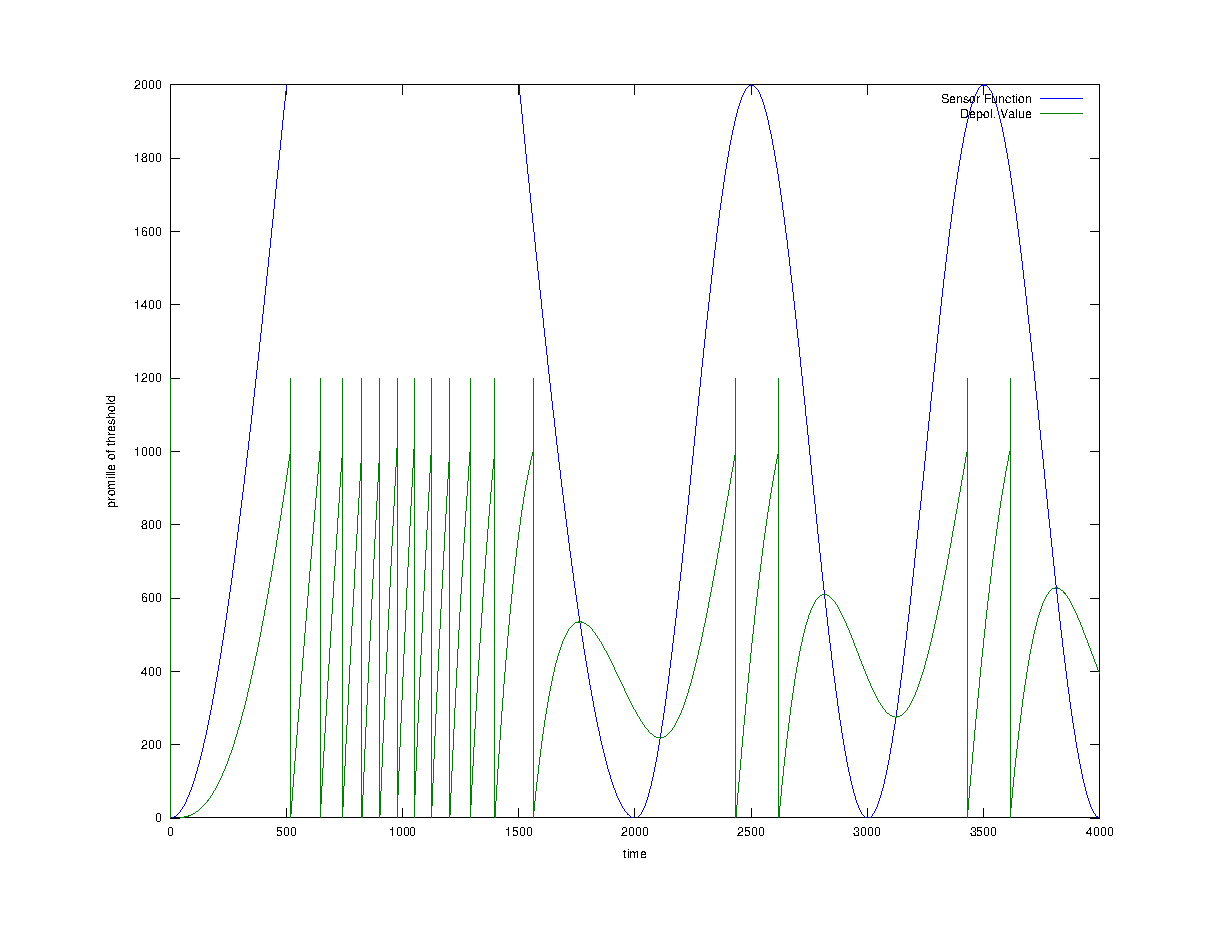
\includegraphics[width=0.95\textwidth]{sensorAuron.eps}
	\caption{Example of the use of a sensor auron. A sensor function is designed to be \mbox{$2\tau (1-cos(\pi \frac{t}{1000}))$} before time $t=1500$. After this it halves the amplitude and doubles the frequency.
			The blue curve represents the sensor function. The green curve represents the ``depolarization'' of the node. Firing is represented by a vertical line in the value curve.
			(Generated by AuroSim)} 
	\label{figSensorAuronExample}
\end{figure}

	The sensor nodes are instances of a class named \emph{s\_sensor\_auron} for the SANN model or \emph{K\_sensor\_auron} for the $\kappa$ANN model.
	In the following text, the \emph{K\_sensor\_auron} will be introduced, but the aspects are general and the presented aspects are valid for both classes. % same goes for the SANN variant of the node.

 	The sensor auron is a specialized auron node, where the activity level of the node varies with some external function.
	This function is called ``the sensor function'', and is possible to design specifically for what is tested for the node.
	In sec. \ref{secComparisonOfMechanismsOfNodeElements} this is used;
		Functions are especially designed to compare different aspects of the SANN node vs. the $\kappa$ANN node. %between the two models.

	Objects of these classes update its activity level each time iteration.
	The activity level, represented by $\kappa$ in $\kappa$ANN, is given by the output of some ``sensor function''.

	The operation of the sensor node is very inspired by biology, where we also have specialized receptor cells responsible for the monitoring of the environment\cite{NeuroscienceExploringTheBrain3edKAP8}.

	\subsubsection{The sensor function is a function pointer}
	The sensor function is the method that ``senses''.
	This can be designed to test certain mechanism of the node.
	
	In fig. \ref{figSensorAuronExample}, this sensor function is set to be a sinusoidal curve with an amplitude of $4 \tau$. 
	At time $t=1500$, the sensor function halves the amplitute and doubles the frequency of the sinusoidal cuve.
	The figure shows the sensor function and the resulting depolarization of the sensor auron.

	The sensor auron class contain a function pointer.
\begin{lstlisting}
double (*pSensorFunction)(void);
\end{lstlisting}
	At the time of construction of each sensor auron object, the constructor takes a function pointer as an argument and assigns its function pointer variable to this value.
	This gives that for a new test case, it is possible to define a new function, and send in the reference to this function to the constructor of the sensor auron.
\begin{lstlisting}
K_sensor_auron::K_sensor_auron(
  std::string sNavn_Arg, double (*pFunk_arg)(void) ) 
     :  K_auron(sNavn_Arg)
{
	// Assign the sensor function:
	pSensorFunction = pFunk_arg;
	// Add to pAllSensorAurons list:
	pAllSensorAurons.push_back(this);

	...
}
\end{lstlisting}

	\subsubsection{Updating The Sensor Auron}
	The static variable \emph{pAllSensorAurons} is a list containing all the sensor aurons.
	After \emph{time\_class::doTask()} iterates time, all sensor aurons(listed in \emph{pAllSensorAurons}) are updated.
	Inspired by biology, the sensing done by the sensor auron happens at the dendrite;
		The sensor auron is updated by sending in the sensed signal to the dendrite's \emph{newSignal()} function.
	%The sensed signal is therefore sent in to the dendrite as the derived of the sensor function. % , before the result is sent in to the \emph{newSignal()} function.


	For the K\_sensor\_auron this gives the code
\begin{lstlisting}
inline void K_sensor_auron::updateSensorValue()
{ 
	// Use two variables, to find the derived.
	dLastSensedValue = dSensedValue;
	dSensedValue = (*pSensorFunction)(); 

	// Use the native mechanism for dendritic integration for the sensor neuron:
	if( dSensedValue != dLastSensedValue){
		changeKappa_derivedArg( dSensedValue-dLastSensedValue );
	}
}
\end{lstlisting}

	%Litt meir, kanskje. Ikkje heilt naudsynt..









